% ............................................................................ %

\documentclass[compress,10pt]{beamer}

\mode<presentation>
{
  \usetheme{Darmstadt}
  \usefonttheme{professionalfonts}
  \setbeamercovered{transparent}
}

\usepackage[english]{babel}
\usepackage[latin1]{inputenc}

\usepackage{graphicx}
\usepackage{url}
\usepackage{pgf}

% ............................................................................ %

\title{The IzPack tutorial}

\subtitle{Getting started with a basic installer for your software.}

\author{Julien~Ponge\inst{1}}

\institute
{
  \inst{1}%
  \texttt{<julien@izforge.com>}\\
  \url{http://izpack.org/}\\
  IzPack project founder and current maintainer.
}

\date{\today}

\pgfdeclareimage[height=0.5cm]{logo}{logo}
\logo{\pgfuseimage{logo}}

\setbeamertemplate{footline}[frame number]
\setbeamertemplate{navigation symbols}{}
\setbeamertemplate{background canvas}[vertical shading][top=blue!10,bottom=white]

\pgfdeclareimage[width=1.5cm,interploate=true]{cc}{cc}
\pgfdeclareimage[width=3cm,interpolate=true]{tree-view}{tree-view}

\pgfdeclareimage[width=9cm,interpolate=true]{panel-hello}{panel-hello}
\pgfdeclareimage[width=9cm,interpolate=true]{panel-info}{panel-info}
\pgfdeclareimage[width=9cm,interpolate=true]{panel-license}{panel-license}
\pgfdeclareimage[width=9cm,interpolate=true]{panel-packs}{panel-packs}
\pgfdeclareimage[width=9cm,interpolate=true]{panel-target}{panel-target}
\pgfdeclareimage[width=9cm,interpolate=true]{panel-install}{panel-install}
\pgfdeclareimage[width=9cm,interpolate=true]{panel-finish}{panel-finish}

\AtBeginSubsection[]
{
  \begin{frame}<beamer>
    \frametitle{Outline}
    \tableofcontents[currentsection,currentsubsection]
  \end{frame}
}

% ............................................................................ %

\begin{document}

% ............................................................................ %

\begin{frame}
  \titlepage
\end{frame}

% ............................................................................ %

\begin{frame}[plain]

\footnotesize

\href{http://www.creativecommons.org/}{\pgfuseimage{cc}}

\vspace{2em}

Copyright \copyright~2004, 2005 Julien \textsc{Ponge} - All Rights Reserved.

\vspace{2em}
\sloppy
This work is licensed under the \textit{Creative Commons
Attribution - NonCommercial - ShareAlike License}. To view a copy of this license,
visit
\href{http://creativecommons.org/licenses/by-nc-sa/2.0/}{\url{http://creativecommons.org/licenses/by-nc-sa/2.0/}}
or send a letter to Creative Commons, 559 Nathan Abbott Way, Stanford,
California 94305, USA.

\end{frame}

% ............................................................................ %

\begin{frame}
  \frametitle{Outline}
  \tableofcontents
\end{frame}

% ............................................................................ %

\section{Introduction}

% ............................................................................ %

\subsection{The IzPack project}

% ................................... %

\begin{frame}

\frametitle{IzWhat ?}

Fast facts:
  \begin{itemize}
    \item An open-sourced Java\texttrademark~-based cross-platform installer
    generator.

    \item Published under the GNU GPL license.

    \item Project started in 2001 by myself, now developed with the help of
    several developers and contributors (\texttt{Thanks.txt} contains about 90
    lines).

    \item Used by various companies and projects around the world (see the
    \href{http://izpack.org/references}{references page}.

    \item Available for about 22 languages.

    \item One of the most active projects at
    \href{http://www.berlios.de/}{BerliOS}.
  \end{itemize}

\end{frame}

% ................................... %

\begin{frame}

\frametitle{Features}

\begin{itemize}

  \item Cross-platform (tested on Win32, Mac OS X, Linux/i386 and FreeBSD/i386).

  \item XML-based, modular and extensible (you choose what your installer will
  be made of).

  \item Integrates with Jakarta Ant.

  \item Can create shortcuts for Win32 and X11 (FreeDesktop.org-compliant
  environments and window managers).

  \item Not dependent on native code (but can use it in a smart way).

  \item Creates uninstallers.

  \item Can get user input, substitute tokens in files, call scripts and much
  more...

\end{itemize}

\end{frame}

% ................................... %

\begin{frame}

\frametitle{Project life}

\begin{itemize}

  \item Online resources:
    \begin{itemize}
      \item hosted on my website at
      \href{http://izpack.org/}{\url{http://izpack.org/}}

      \item \href{http://www.berlios.de/}{BerliOS} hosts the developer tools
      (CVS, SVN, bugs tracking, wiki, mailing-lists, file releases, FTP, ...).
    \end{itemize}

    \item The development is very open and contributions are always welcome.

    \item Major releases (ex: $3.7.x$) are maintained in branches while the
    development occurs in \texttt{CVS HEAD}.

    \item Minor releases occur depending on fixes inclusion.

    \item Major releases happen depending on new features inclusion.

\end{itemize}

\end{frame}

% ............................................................................ %

\subsection{Technical overview}

\begin{frame}

\frametitle{IzPack}

\begin{columns}

  \begin{column}{6.5cm}
  \begin{itemize}

    \item An installer is described by an \textsl{XML installation file} that:
      \begin{itemize}
        \item arranges files into \textsl{packs}
        \item can be customized by some resources (depending on what you choose).
      \end{itemize}

    \item The compiler takes the XML file as its input to build an installer as
    an \textsl{executable Jar} archive.

  \end{itemize}
  \end{column}

  \begin{column}{4cm}
  
\includegraphics[width=4cm,angle=270]{izpack-overview}
  \end{column}

\end{columns}

\end{frame}

% ................................... %

\begin{frame}

\frametitle{Installers}

\begin{columns}

  \begin{column}{6.5cm}
  \begin{itemize}

    \item An installer contains:
      \begin{itemize}
        \item the real files in packs
        \item the langpacks.
      \end{itemize}

    \item An installer offers a set of panels that define the steps to perform
    an installation.

    \item Resources can be needed by panels and GUI preferences can change the
    look depending on the OS (size, L\&F, ...).

  \end{itemize}
  \end{column}

  \begin{column}{4cm}
  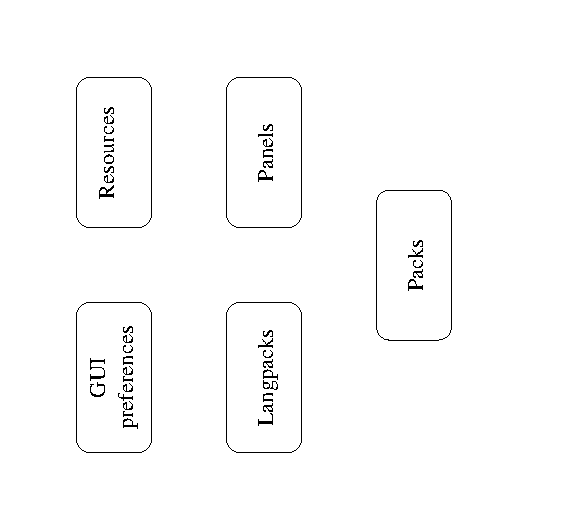
\includegraphics[width=4cm,angle=270]{installers-overview}
  \end{column}

\end{columns}

\end{frame}

% ............................................................................ %

\section{Making an installer}

% ............................................................................ %

\subsection{Preliminary steps}

\begin{frame}

\frametitle{Laying out the files and folders}

\begin{columns}

  \begin{column}{7cm}
  \begin{itemize}

    \item Put your files in a folder. Try to make it easy to split the
    files tree into packs (for instance put the files of a pack into a small set
    of subfolders).

    \item Think about which files and folders your packs will be made of.

    \item Decide which packs will be mandatory and which packs will be optional.

  \end{itemize}
  \end{column}

  \begin{column}{3cm}
  \pgfuseimage{tree-view}
  \end{column}

\end{columns}

\end{frame}

% ................................... %

\begin{frame}

\frametitle{Installation panels flow}

\begin{itemize}

  \item Panels define the installation steps. Several panels are available, some
  even do the same functional task.
  \alert{You decide which panels you want and in which order.}

  \item For this tutorial, we will use the following panels:
    \begin{enumerate}

      \item \textsl{HelloPanel}: welcome our user to the installation process

      \item \textsl{HTMLInfoPanel}: display some informations with a structured
      text

      \item \textsl{LicencePanel}: the legal terms that must be agreed to reach
      the next installation steps

      \item \textsl{PacksPanel}: allow the user to pick the packs that she/he wants
      to install or not

      \item \textsl{TargetPanel}: choose where to install the files

      \item \textsl{InstallPanel}: performs the actual files installation

      \item \textsl{SimpleFinishPanel}: conclude the installation with a success.

    \end{enumerate}

\end{itemize}

\end{frame}

% ................................... %

\begin{frame}

\frametitle{Panels flow illustrated}

\begin{overprint}

  \onslide<1>\textsl{HelloPanel}\\
  
  \pgfuseimage{panel-hello}
  
  \onslide<2>\textsl{HTMLInfoPanel}\\
  
  \pgfuseimage{panel-info}
  
  \onslide<3>\textsl{LicencePanel}\\
  
  \pgfuseimage{panel-license}
  
  \onslide<4>\textsl{PacksPanel} (here \textit{ImgPacksPanel})\\
  
  \pgfuseimage{panel-packs}
  
  \onslide<5>\textsl{TargetPanel}\\
  
  \pgfuseimage{panel-target}
  
  \onslide<6>\textsl{InstallPanel}\\
  
  \pgfuseimage{panel-install}
  
  \onslide<7>\textsl{SimpleFinishPanel}\\
  
  \pgfuseimage{panel-finish}

\end{overprint}

\end{frame}

% ............................................................................ %

\subsection{Creating the installation files}

\begin{frame}[containsverbatim]

\frametitle{Basic installation XML file canvas}

Here is a global view of what our file will look like:

\begin{block}{\texttt{MyApp-install.xml}}
\small
\begin{verbatim}
<installation version="1.0">

    <info> (...) </info>
    <guiprefs (...)> (...) </guiprefs>
    <locale> (...) </locale>
    <resources> (...) </resources>
    <panels> (...) </panels>
    <packs> (...) </packs>

</installation>
\end{verbatim}
\end{block}

\end{frame}

% ................................... %

\begin{frame}[containsverbatim]

\frametitle{Global informations}

We will specify here:
  \begin{itemize}
      \item the authors of the application to install
      \item the application name, version and url
      \item the minimum Java\texttrademark~ version required (optional).
  \end{itemize}

\begin{block}{The \textsl{info} section}
\tiny
\begin{verbatim}
<info>
    <appname>MyApp</appname>
    <appversion>1.2.3</appversion>
    <authors>
        <author name="Snoopy" email="snoopy@myapp.org" />
        <author name="Foo Bar" email="foo@bar.org" />
    </authors>
    <url>http://www.myapp.org/</url>
    <javaversion>1.4</javaversion>
</info>
\end{verbatim}
\end{block}

\end{frame}

% ................................... %

\begin{frame}[containsverbatim]

\frametitle{GUI tweakings}

\begin{itemize}

  \item We can customise the default size.

  \item We can specify a Look \& Feel for a given OS, including:
    \begin{itemize}
      \item Metal (hum hum ...)
      \item Kunststoff, Metouia, Liquid
      \item JGoodies variants.
    \end{itemize}

  \item The default is to pick the native emulation L\&F.

\end{itemize}

\begin{block}{The \textsl{guiprefs} section}
\tiny
\begin{verbatim}
<guiprefs height="600" resizable="yes" width="800">
    <laf name="metouia">
        <os family="unix" />
    </laf>
</guiprefs>
\end{verbatim}
\end{block}

\end{frame}

% ................................... %

\begin{frame}[containsverbatim]

\frametitle{Choosing the available languages}

This step is quite easy. Just pick the ISO3 codes among the available languages,
for instance:

\begin{block}{The \textsl{locale} section}
\tiny
\begin{verbatim}
<locale>
    <langpack iso3="eng"/>
    <langpack iso3="fra"/>
    <langpack iso3="deu"/>
    <langpack iso3="ita"/>
    <langpack iso3="jpn"/>
    <langpack iso3="spa"/>
</locale>
\end{verbatim}
\end{block}

\end{frame}

% ................................... %

\begin{frame}[containsverbatim]

\frametitle{Including the needed resources}

\begin{itemize}

  \item Each panel needs resources (see the IzPack documentation). A resource
  associates a path to a file and an identifier.

  \item Here, we have the following resources:
    \begin{itemize}
      \item the text for \textsl{HTMLInfoPanel}
      \item the legal terms for \textsl{LicencePanel}
      \item an optional picture for the language selection box.
    \end{itemize}

\end{itemize}

\begin{block}{The \textsl{resources} section}
\tiny
\begin{verbatim}
<resources>
    <res src="install-readme.html" id="HTMLInfoPanel.info"/>
    <res src="Licence.txt" id="LicencePanel.licence"/>
    <res src="langsel.jpg" id="installer.langsel.img"/>
</resources>
\end{verbatim}
\end{block}

\end{frame}

% ................................... %

\begin{frame}[containsverbatim]

\frametitle{Specifying the panels}

Simply put the panels names in the obvious order:

\begin{block}{The \textsl{panels} section}
\tiny
\begin{verbatim}
<panels>
    <panel classname="HelloPanel"/>
    <panel classname="HTMLInfoPanel"/>
    <panel classname="LicencePanel"/>
    <panel classname="PacksPanel"/>
    <panel classname="TargetPanel"/>
    <panel classname="InstallPanel"/>
    <panel classname="SimpleFinishPanel"/>
</panels>
\end{verbatim}
\end{block}

\end{frame}

% ................................... %

\begin{frame}[containsverbatim]

\frametitle{Making the packs}

\begin{itemize}

  \item We use the smart Ant filesets syntax to pick the files contained in 
  each pack.

  \item Target directories are specified. \alert{\texttt{\small\$INSTALL\_PATH}
  identifies the path chosen from \textsl{TargetPanel}}.

\end{itemize}

\begin{block}{The \textsl{packs} section}
\tiny
\begin{verbatim}
<packs>
    <pack name="Core" required="yes">
        <description>MyApp core files.</description>
        <fileset dir="" targetdir="$INSTALL_PATH">
          <include name="*.txt" />
          <include name="bin/**/*" />
          <include name="lib/**/*" />
        </fileset>
    </pack>
    (...)
</packs>
\end{verbatim}
\end{block}

\end{frame}

% ............................................................................ %

\subsection{Building the installer}

\begin{frame}

\frametitle{Ant integration}

\begin{itemize}

  \item Ant is perfect for software tasks automation.

  \item IzPack can be integrated with Ant in a simple and elegant manner.

  \item IzPack needs the following informations (the same holds true for a
  command-line invocation):
    \begin{itemize}
      \item the input installation XML file

      \item the name of the output installer Jar file

      \item the kind of installer (standard or web-based)

      \item the base directory, to resolve the relative paths specified for the
      various files of the XML installation file (files, resources, ...)

      \item the directory where IzPack is installed.
    \end{itemize}

\end{itemize}

\end{frame}

% ................................... %

\begin{frame}[containsverbatim]

\frametitle{Calling IzPack from Ant}

\begin{alertblock}{Warning}
Make the IzPack compiler jar available in the classpath before you call Ant.
\end{alertblock}

\begin{block}{Make the task available}
\tiny
\begin{verbatim}
<taskdef name="izpack" classpath="${izpack.dir}/lib/compiler.jar"
         classname="com.izforge.izpack.ant.IzPackTask"/>
\end{verbatim}
\end{block}

\begin{block}{Call the IzPack task}
\tiny
\begin{verbatim}
<izpack input="MyApp-install.xml"
        output="${dist.dir}/MyApp-install-${ver}.${rel}.jar"
        installerType="standard" basedir="${dist.dir}"
        izPackDir="${izpack.dir}/"/>
\end{verbatim}
\end{block}

\end{frame}

% ............................................................................ %

\section{Conclusion}

\begin{frame}

\frametitle{Summary}

\begin{itemize}

  \item You have now made a simple installer for your application. You should
  now feel more confident with IzPack, however you can get much more from it.

  \item You can now try some more advanced features (such as desktop shortcuts
  generation or scripts token replacement) or play with some other panels as
  well.

  \item The following resources will be of a great help:
  \begin{itemize}

    \item the IzPack documentation

    \item the \href{http://openfacts.berlios.de/index-en.phtml?title=IzPack}{
    wiki} at BerliOS

    \item the \href{http://developer.berlios.de/mail/?group_id=1408}{
    mailing-lists archives}

    \item real-life examples (such as IzPack itself or open-source projects that
    use it).

  \end{itemize}

\end{itemize}

\end{frame}

\begin{frame}

\frametitle{Supporting IzPack}

If IzPack is useful to you and/or your company, please consider supporting it
financially. Just think about how expensive are its proprietary competitors...

\begin{itemize}

  \item I accept donations through PayPal with my email address
  \small{\url{julien@izforge.com}}.

  \item Missing a feature ? Then you can offer a bounty to an IzPack developer
  for implementing it. Ask for the feature and see if a developer wants to make
  it for a donation that you can negotiate at your own discretion with her/him.

\end{itemize}

\end{frame}

\begin{frame}

\frametitle{Credits}

\begin{itemize}

  \item The \href{http://latex-beamer.sf.net/}{\LaTeX~Beamer} class.

  \item The \href{http://www.berlios.de/}{BerliOS} crew.

  \item The numerous past and present IzPack developers and contributors.

\end{itemize}

\end{frame}

% ............................................................................ %

\end{document}


